\section{Algorithmic Optimizations} \label{sec:algopti}
\subsection{\acrfull{gemm}}
It is a common way to process \acrshort{cnn} on \acrshort{cpu} and \acrshort{gpu}. We convert the convolution as a matrix-vector multiplication.  The process of a convolution layer can be observed on Figure \ref{fig:gemm}.
However, this approach is not suggested for \acrshort{fpga}: \cite{sze_efficient_2017, zhu_efficient_2020} point out that the \acrshort{fm}s have to be copied multiple times when flattened to a vector. It leads to a huge memory footprint and either ineffiency in storage or complex memory management access patterns.
\begin{figure}
    \centering
    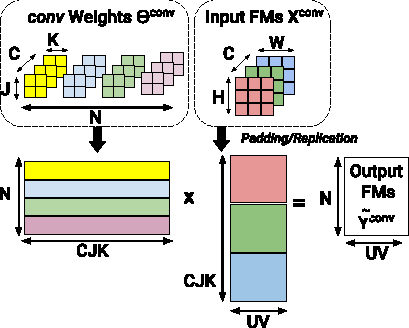
\includegraphics[width=0.5\textwidth]{Images/gemm.pdf}
    \caption{\acrshort{gemm} base processing on conv layer}
    \label{fig:gemm}
\end{figure}
\subsection{Winograd Transform}
The Winograd minimal filter algorithm is first introduced by \cite{winograd_arithmetic_1980}. In Winograd filtering, data is processed by blocs referred as \textit{tiles}, as following:
\begin{itemize}
    \item An input \acrshort{fm} tile $g$ of size $(N_{ix} \times N_{iy})$ is pre-processed: $\tilde{g} = \boldsymbol{G^{T}} g \boldsymbol{G} $, where $\boldsymbol{G}$ is a transformation matrix defined in the Winograd Algorithm \cite{winograd_arithmetic_1980}.
    \item In a same way, $d$, the filter of size $(K_x \times K_y)$ is transformed into $\tilde{d}$: $\tilde{d} = \boldsymbol{B^{T}} d \boldsymbol{B}$ , where $\boldsymbol{B}$ is a transformation matrix defined in the Winograd Algorithm \cite{winograd_arithmetic_1980}.
    \item The output tile $Y$ of the Winograd Filtering algorithm, denoted $F(N_{ix} \times N_{iy}, K_x \times K_y)$ is computed using equation \ref{eqn:winograd}, where $\boldsymbol{A}$ is a transformation matrix defined in the Winograd Algorithm \cite{winograd_arithmetic_1980} and $\odot$ indicates element-wise multiplication.
\end{itemize}
\begin{equation}
\label{eqn:winograd}
Y = \boldsymbol{A^{T}} [ \ \tilde{g} \odot \tilde{d} \ ] \boldsymbol{A}
\end{equation}
\cite{lavin_fast_2015} demonstrated that Winograd convolution is efficient when the kernel is small ($K_* \leq 3$) and the number of multiplication can be reduced by a factor of $2.25 \times$ (in returns the number of addition is increased). According to \cite{sandler_mobilenetv2_2019}, $3 \times 3$ kernel is a standard for modern networks, which leads that Winograd Transform can be applied in modern network. However, we can only apply this computational transform to convolutions when the stride is equal to 1.
\subsection{\acrfull{fft}}
The \acrshort{fft} is an algorithm to transform the 2D convolution into element-wise multiplication in the frequency domain. The equation is observed at equation \ref{eqn:fft}
\begin{equation}
\label{eqn:fft}
conv2D(FM_{I}[ic], K[oc, ic]) = IFFT( FFT(FM_{I}[ic]) \odot FFT(K[oc, ic]) )
\end{equation}
The arithmetic complexity of the 2D convolution can be reduced to $O(N_{ix}^2 log_2(N_{ix}))$ \cite{jong_hwan_ko_design_2017} and the computational complexity of the \acrshort{fft} can be reduced to $O(N_{ix} log_2(K_{x}))$ using the Overlap-and-Add Method \cite{w_smith_scientist_1997}.
However, the \acrshort{fft} finds its interest when kernel are large \cite{lavin_fast_2015} ($K_* \geq 5$), which is not a standard kernel size according to \cite{sandler_mobilenetv2_2019}.
